\documentclass[]{article}
\usepackage{lmodern}
\usepackage{amssymb,amsmath}
\usepackage{ifxetex,ifluatex}
\usepackage{fixltx2e} % provides \textsubscript
\ifnum 0\ifxetex 1\fi\ifluatex 1\fi=0 % if pdftex
  \usepackage[T1]{fontenc}
  \usepackage[utf8]{inputenc}
\else % if luatex or xelatex
  \ifxetex
    \usepackage{mathspec}
  \else
    \usepackage{fontspec}
  \fi
  \defaultfontfeatures{Ligatures=TeX,Scale=MatchLowercase}
\fi
% use upquote if available, for straight quotes in verbatim environments
\IfFileExists{upquote.sty}{\usepackage{upquote}}{}
% use microtype if available
\IfFileExists{microtype.sty}{%
\usepackage{microtype}
\UseMicrotypeSet[protrusion]{basicmath} % disable protrusion for tt fonts
}{}
\usepackage[margin=1in]{geometry}
\usepackage{hyperref}
\hypersetup{unicode=true,
            pdftitle={Reproducible Research: Peer Assessment 1},
            pdfauthor={Juan C. López Tavera},
            pdfborder={0 0 0},
            breaklinks=true}
\urlstyle{same}  % don't use monospace font for urls
\usepackage{color}
\usepackage{fancyvrb}
\newcommand{\VerbBar}{|}
\newcommand{\VERB}{\Verb[commandchars=\\\{\}]}
\DefineVerbatimEnvironment{Highlighting}{Verbatim}{commandchars=\\\{\}}
% Add ',fontsize=\small' for more characters per line
\usepackage{framed}
\definecolor{shadecolor}{RGB}{248,248,248}
\newenvironment{Shaded}{\begin{snugshade}}{\end{snugshade}}
\newcommand{\KeywordTok}[1]{\textcolor[rgb]{0.13,0.29,0.53}{\textbf{#1}}}
\newcommand{\DataTypeTok}[1]{\textcolor[rgb]{0.13,0.29,0.53}{#1}}
\newcommand{\DecValTok}[1]{\textcolor[rgb]{0.00,0.00,0.81}{#1}}
\newcommand{\BaseNTok}[1]{\textcolor[rgb]{0.00,0.00,0.81}{#1}}
\newcommand{\FloatTok}[1]{\textcolor[rgb]{0.00,0.00,0.81}{#1}}
\newcommand{\ConstantTok}[1]{\textcolor[rgb]{0.00,0.00,0.00}{#1}}
\newcommand{\CharTok}[1]{\textcolor[rgb]{0.31,0.60,0.02}{#1}}
\newcommand{\SpecialCharTok}[1]{\textcolor[rgb]{0.00,0.00,0.00}{#1}}
\newcommand{\StringTok}[1]{\textcolor[rgb]{0.31,0.60,0.02}{#1}}
\newcommand{\VerbatimStringTok}[1]{\textcolor[rgb]{0.31,0.60,0.02}{#1}}
\newcommand{\SpecialStringTok}[1]{\textcolor[rgb]{0.31,0.60,0.02}{#1}}
\newcommand{\ImportTok}[1]{#1}
\newcommand{\CommentTok}[1]{\textcolor[rgb]{0.56,0.35,0.01}{\textit{#1}}}
\newcommand{\DocumentationTok}[1]{\textcolor[rgb]{0.56,0.35,0.01}{\textbf{\textit{#1}}}}
\newcommand{\AnnotationTok}[1]{\textcolor[rgb]{0.56,0.35,0.01}{\textbf{\textit{#1}}}}
\newcommand{\CommentVarTok}[1]{\textcolor[rgb]{0.56,0.35,0.01}{\textbf{\textit{#1}}}}
\newcommand{\OtherTok}[1]{\textcolor[rgb]{0.56,0.35,0.01}{#1}}
\newcommand{\FunctionTok}[1]{\textcolor[rgb]{0.00,0.00,0.00}{#1}}
\newcommand{\VariableTok}[1]{\textcolor[rgb]{0.00,0.00,0.00}{#1}}
\newcommand{\ControlFlowTok}[1]{\textcolor[rgb]{0.13,0.29,0.53}{\textbf{#1}}}
\newcommand{\OperatorTok}[1]{\textcolor[rgb]{0.81,0.36,0.00}{\textbf{#1}}}
\newcommand{\BuiltInTok}[1]{#1}
\newcommand{\ExtensionTok}[1]{#1}
\newcommand{\PreprocessorTok}[1]{\textcolor[rgb]{0.56,0.35,0.01}{\textit{#1}}}
\newcommand{\AttributeTok}[1]{\textcolor[rgb]{0.77,0.63,0.00}{#1}}
\newcommand{\RegionMarkerTok}[1]{#1}
\newcommand{\InformationTok}[1]{\textcolor[rgb]{0.56,0.35,0.01}{\textbf{\textit{#1}}}}
\newcommand{\WarningTok}[1]{\textcolor[rgb]{0.56,0.35,0.01}{\textbf{\textit{#1}}}}
\newcommand{\AlertTok}[1]{\textcolor[rgb]{0.94,0.16,0.16}{#1}}
\newcommand{\ErrorTok}[1]{\textcolor[rgb]{0.64,0.00,0.00}{\textbf{#1}}}
\newcommand{\NormalTok}[1]{#1}
\usepackage{longtable,booktabs}
\usepackage{graphicx,grffile}
\makeatletter
\def\maxwidth{\ifdim\Gin@nat@width>\linewidth\linewidth\else\Gin@nat@width\fi}
\def\maxheight{\ifdim\Gin@nat@height>\textheight\textheight\else\Gin@nat@height\fi}
\makeatother
% Scale images if necessary, so that they will not overflow the page
% margins by default, and it is still possible to overwrite the defaults
% using explicit options in \includegraphics[width, height, ...]{}
\setkeys{Gin}{width=\maxwidth,height=\maxheight,keepaspectratio}
\IfFileExists{parskip.sty}{%
\usepackage{parskip}
}{% else
\setlength{\parindent}{0pt}
\setlength{\parskip}{6pt plus 2pt minus 1pt}
}
\setlength{\emergencystretch}{3em}  % prevent overfull lines
\providecommand{\tightlist}{%
  \setlength{\itemsep}{0pt}\setlength{\parskip}{0pt}}
\setcounter{secnumdepth}{0}
% Redefines (sub)paragraphs to behave more like sections
\ifx\paragraph\undefined\else
\let\oldparagraph\paragraph
\renewcommand{\paragraph}[1]{\oldparagraph{#1}\mbox{}}
\fi
\ifx\subparagraph\undefined\else
\let\oldsubparagraph\subparagraph
\renewcommand{\subparagraph}[1]{\oldsubparagraph{#1}\mbox{}}
\fi

%%% Use protect on footnotes to avoid problems with footnotes in titles
\let\rmarkdownfootnote\footnote%
\def\footnote{\protect\rmarkdownfootnote}

%%% Change title format to be more compact
\usepackage{titling}

% Create subtitle command for use in maketitle
\newcommand{\subtitle}[1]{
  \posttitle{
    \begin{center}\large#1\end{center}
    }
}

\setlength{\droptitle}{-2em}
  \title{Reproducible Research: Peer Assessment 1}
  \pretitle{\vspace{\droptitle}\centering\huge}
  \posttitle{\par}
  \author{Juan C. López Tavera}
  \preauthor{\centering\large\emph}
  \postauthor{\par}
  \date{}
  \predate{}\postdate{}


\begin{document}
\maketitle

\subsection{Introduction}\label{introduction}

This is the peer-graded assignment for the Reproducible Research Course
by Johns Hopkins University at Coursera, which is the 5th out of 10
courses in the
\href{https://www.coursera.org/specializations/jhu-data-science}{Data
Science Specialization}.

The objective of this assignment is to make a reproducible report of an
individual's activity over a two month period, measured in number of
steps. The report will be generated using
\href{https://yihui.name/knitr/}{knitr}.

As provided in Professor Peng's
\href{https://github.com/rdpeng/RepData_PeerAssessment1}{original
repository}, this repository is self-contained --- all data and
assignment instructions necessary to reproduce this work are available
in the same place.

\subsubsection{Setting up the report}\label{setting-up-the-report}

First, we need to setup the report options using, and install ---if
necessary--- and load all the required packages to successfully complete
this assignment.

\begin{Shaded}
\begin{Highlighting}[]
\NormalTok{## Loading the necessary package for reproducing the assingment}
\ControlFlowTok{if}\NormalTok{ (}\OperatorTok{!}\KeywordTok{require}\NormalTok{(knitr)) \{}
    \KeywordTok{install.packages}\NormalTok{(}\StringTok{"knitr"}\NormalTok{)}
\NormalTok{\}}
\KeywordTok{library}\NormalTok{(knitr)}

\ControlFlowTok{if}\NormalTok{ (}\OperatorTok{!}\KeywordTok{require}\NormalTok{(tidyverse)) \{}
    \KeywordTok{install.packages}\NormalTok{(}\StringTok{"tidyverse"}\NormalTok{)}
\NormalTok{\}}
\KeywordTok{library}\NormalTok{(tidyverse)}

\NormalTok{## Setting up all code chunks according to the assignment specs}
\NormalTok{knitr}\OperatorTok{::}\NormalTok{opts_chunk}\OperatorTok{$}\KeywordTok{set}\NormalTok{(}
    \DataTypeTok{eval =} \OtherTok{TRUE}\NormalTok{,}
    \DataTypeTok{echo =} \OtherTok{TRUE}\NormalTok{,}
    \DataTypeTok{tidy =} \OtherTok{TRUE}\NormalTok{,}
    \DataTypeTok{results =} \StringTok{"markup"}\NormalTok{,}
    \DataTypeTok{include =} \OtherTok{TRUE}\NormalTok{,}
    \DataTypeTok{message =} \OtherTok{FALSE}\NormalTok{,}
    \DataTypeTok{warning =} \OtherTok{FALSE}\NormalTok{,}
    \DataTypeTok{knitr.table.format =} \StringTok{"markdown"}\NormalTok{, }
    \DataTypeTok{tidy.opts =} \KeywordTok{list}\NormalTok{(}\DataTypeTok{width.cutoff =} \DecValTok{80}\NormalTok{), }
    \DataTypeTok{fig.align =} \StringTok{"center"}\NormalTok{, }
    \DataTypeTok{fig.path =} \StringTok{"figure/"}\NormalTok{, }
    \DataTypeTok{highlight =} \OtherTok{TRUE}
\NormalTok{)}
\end{Highlighting}
\end{Shaded}

\subsection{Loading and preprocessing the
data}\label{loading-and-preprocessing-the-data}

\begin{verbatim}
Instructions: 
Show any code that is needed to
1. Load the data (i.e. read.csv())
2. Process/transform the data (if necessary) into a format suitable for your analysis
\end{verbatim}

In the original repository, the data set is compressed in a ZIP file,
which we unzip ---if necessary--- and load the resulting CSV file into
the working environment.

No pre-processing was necessary for this data set, as it is already
tidy.

\begin{Shaded}
\begin{Highlighting}[]
\NormalTok{## If necessary, unzipping the data file, and loading it}
\ControlFlowTok{if}\NormalTok{ (}\OperatorTok{!}\KeywordTok{file.exists}\NormalTok{(}\StringTok{"activity.csv"}\NormalTok{) }\OperatorTok{&}\StringTok{ }\KeywordTok{file.exists}\NormalTok{(}\StringTok{"activity.zip"}\NormalTok{)) \{}
    \KeywordTok{unzip}\NormalTok{(}\StringTok{"activity.zip"}\NormalTok{)}
\NormalTok{    activity.data <-}\StringTok{ }\KeywordTok{read_csv}\NormalTok{(}\DataTypeTok{file =} \StringTok{"activity.csv"}\NormalTok{)}
\NormalTok{\} }\ControlFlowTok{else} \ControlFlowTok{if}\NormalTok{ (}\KeywordTok{file.exists}\NormalTok{(}\StringTok{"activity.csv"}\NormalTok{)) \{}
\NormalTok{    activity.data <-}\StringTok{ }\KeywordTok{read_csv}\NormalTok{(}\DataTypeTok{file =} \StringTok{"activity.csv"}\NormalTok{)}
\NormalTok{\} }\ControlFlowTok{else}\NormalTok{ \{}
    \KeywordTok{message}\NormalTok{(}\StringTok{"Activity Monitoring Data (default) from Rep Research course was not found"}\NormalTok{)}
\NormalTok{\}}
\end{Highlighting}
\end{Shaded}

\subsection{What is mean total number of steps taken per
day?}\label{what-is-mean-total-number-of-steps-taken-per-day}

\begin{verbatim}
Instrunctions:
For this part of the assignment, you can ignore the missing values in the dataset.  
1. Make a histogram of the total number of steps taken each day.
2. Calculate and report the **mean** and **median** total number of steps taken per day.
\end{verbatim}

We want to know the distribution of the number of steps taken each day,
which we can observe in a histogram generated using ggplot2.

In the figure below, we can observe the histogram of the number of steps
taken each day, with an overlayed density plot.

\begin{Shaded}
\begin{Highlighting}[]
\NormalTok{steps.day.df <-}\StringTok{ }\NormalTok{activity.data }\OperatorTok\StringTok{ }\KeywordTok{group_by}\NormalTok{(date) }\OperatorTok\StringTok{ }\KeywordTok{summarise}\NormalTok{(}\DataTypeTok{steps =} \KeywordTok{sum}\NormalTok{(steps))}

\NormalTok{mean.median.steps <-}\StringTok{ }\NormalTok{steps.day.df }\OperatorTok\StringTok{ }\KeywordTok{summarise}\NormalTok{(}\DataTypeTok{Mean =} \KeywordTok{round}\NormalTok{(}\KeywordTok{mean}\NormalTok{(steps, }\DataTypeTok{na.rm =} \OtherTok{TRUE}\NormalTok{)), }
    \DataTypeTok{Median =} \KeywordTok{round}\NormalTok{(}\KeywordTok{median}\NormalTok{(steps, }\DataTypeTok{na.rm =} \OtherTok{TRUE}\NormalTok{))) }\OperatorTok\StringTok{ }\KeywordTok{gather}\NormalTok{()}

\KeywordTok{ggplot}\NormalTok{(}\DataTypeTok{data =}\NormalTok{ steps.day.df, }\DataTypeTok{mapping =} \KeywordTok{aes}\NormalTok{(}\DataTypeTok{x =}\NormalTok{ steps, }\DataTypeTok{y =}\NormalTok{ ..density..)) }\OperatorTok{+}\StringTok{ }\KeywordTok{geom_histogram}\NormalTok{(}\KeywordTok{aes}\NormalTok{(}\DataTypeTok{weight =}\NormalTok{ steps), }
    \DataTypeTok{fill =} \StringTok{"steelblue"}\NormalTok{, }\DataTypeTok{colour =} \StringTok{"white"}\NormalTok{, }\DataTypeTok{alpha =} \FloatTok{0.8}\NormalTok{) }\OperatorTok{+}\StringTok{ }\KeywordTok{geom_density}\NormalTok{(}\DataTypeTok{fill =} \StringTok{"steelblue"}\NormalTok{, }
    \DataTypeTok{colour =} \OtherTok{NA}\NormalTok{, }\DataTypeTok{alpha =} \FloatTok{0.2}\NormalTok{) }\OperatorTok{+}\StringTok{ }\KeywordTok{ggtitle}\NormalTok{(}\KeywordTok{list}\NormalTok{(}\DataTypeTok{title =} \StringTok{"Total Number of Steps"}\NormalTok{, }\DataTypeTok{subtitle =} \StringTok{"Distribution of Total Number of Steps Taken Each Day"}\NormalTok{, }
    \DataTypeTok{x =} \StringTok{"Steps"}\NormalTok{, }\DataTypeTok{y =} \StringTok{"Density"}\NormalTok{)) }\OperatorTok{+}\StringTok{ }\KeywordTok{geom_vline}\NormalTok{(}\DataTypeTok{data =}\NormalTok{ mean.median.steps, }\KeywordTok{aes}\NormalTok{(}\DataTypeTok{xintercept =}\NormalTok{ value, }
    \DataTypeTok{linetype =}\NormalTok{ key), }\DataTypeTok{size =} \FloatTok{0.5}\NormalTok{, }\DataTypeTok{alpha =} \FloatTok{0.8}\NormalTok{, }\DataTypeTok{colour =} \KeywordTok{c}\NormalTok{(}\StringTok{"salmon"}\NormalTok{, }\StringTok{"royalblue"}\NormalTok{)) }\OperatorTok{+}\StringTok{ }
\StringTok{    }\KeywordTok{scale_linetype_discrete}\NormalTok{(}\DataTypeTok{name =} \StringTok{"Number of Steps"}\NormalTok{) }\OperatorTok{+}\StringTok{ }\KeywordTok{theme_bw}\NormalTok{()}
\end{Highlighting}
\end{Shaded}

\begin{center}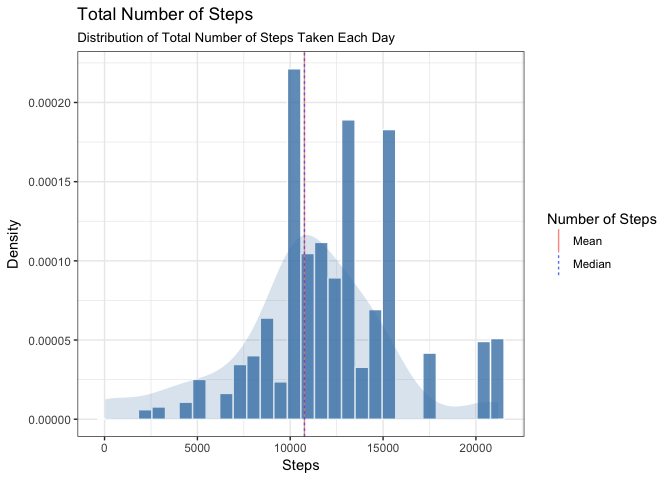
\includegraphics{figure/histogram-1} \end{center}

We want to know basic statistics about the number of steps, which are
also depicted in the following table:

\begin{Shaded}
\begin{Highlighting}[]
\NormalTok{steps.day.df }\OperatorTok\StringTok{ }\KeywordTok{summarise}\NormalTok{(}\StringTok{`}\DataTypeTok{Mean number of steps taken per day}\StringTok{`}\NormalTok{ =}\StringTok{ }\KeywordTok{round}\NormalTok{(}\KeywordTok{mean}\NormalTok{(steps, }
    \DataTypeTok{na.rm =} \OtherTok{TRUE}\NormalTok{)), }\StringTok{`}\DataTypeTok{Median number of steps taken per day}\StringTok{`}\NormalTok{ =}\StringTok{ }\KeywordTok{round}\NormalTok{(}\KeywordTok{median}\NormalTok{(steps, }
    \DataTypeTok{na.rm =} \OtherTok{TRUE}\NormalTok{))) }\OperatorTok\StringTok{ }\KeywordTok{kable}\NormalTok{(}\DataTypeTok{align =} \StringTok{"c"}\NormalTok{)}
\end{Highlighting}
\end{Shaded}

\begin{longtable}[]{@{}cc@{}}
\toprule
Mean number of steps taken per day & Median number of steps taken per
day\tabularnewline
\midrule
\endhead
10766 & 10765\tabularnewline
\bottomrule
\end{longtable}

\subsection{What is the average daily activity
pattern?}\label{what-is-the-average-daily-activity-pattern}

\begin{verbatim}
Instructions:
1. Make a time series plot (i.e. `type = "l"`) of the 5-minute interval (x-axis) and the average number of steps taken, averaged across all days (y-axis).
2. Which 5-minute interval, on average across all the days in the dataset, contains the maximum number of steps?
\end{verbatim}

We also want to know the daily activity pattern, which is how many steps
---averaged across all days--- are taken during the day.

For this purpose, we create a line plot, using ggplot2, shown below.

\begin{Shaded}
\begin{Highlighting}[]
\NormalTok{avg.steps.day <-}\StringTok{ }\NormalTok{activity.data }\OperatorTok\StringTok{ }\KeywordTok{group_by}\NormalTok{(interval) }\OperatorTok\StringTok{ }\KeywordTok{summarise}\NormalTok{(}\DataTypeTok{steps =} \KeywordTok{round}\NormalTok{(}\KeywordTok{mean}\NormalTok{(steps, }
    \DataTypeTok{na.rm =} \OtherTok{TRUE}\NormalTok{))) }\OperatorTok\StringTok{ }\KeywordTok{filter}\NormalTok{(}\OperatorTok{!}\KeywordTok{is.nan}\NormalTok{(steps))}

\NormalTok{max.steps <-}\StringTok{ }\NormalTok{avg.steps.day[}\KeywordTok{which.max}\NormalTok{(avg.steps.day}\OperatorTok{$}\NormalTok{steps), ]}

\KeywordTok{ggplot}\NormalTok{(}\DataTypeTok{data =}\NormalTok{ avg.steps.day, }\DataTypeTok{mapping =} \KeywordTok{aes}\NormalTok{(}\DataTypeTok{x =}\NormalTok{ interval, }\DataTypeTok{y =}\NormalTok{ steps)) }\OperatorTok{+}\StringTok{ }\KeywordTok{geom_line}\NormalTok{(}\DataTypeTok{size =} \FloatTok{0.5}\NormalTok{, }
    \DataTypeTok{colour =} \StringTok{"steelblue"}\NormalTok{, }\DataTypeTok{alpha =} \FloatTok{0.9}\NormalTok{) }\OperatorTok{+}\StringTok{ }\KeywordTok{ggtitle}\NormalTok{(}\KeywordTok{list}\NormalTok{(}\DataTypeTok{title =} \StringTok{"Daily Activity Pattern"}\NormalTok{, }
    \DataTypeTok{subtitle =} \StringTok{"Average number of steps taken by 5-min interval, across all days"}\NormalTok{, }
    \DataTypeTok{y =} \StringTok{"Number of Steps"}\NormalTok{, }\DataTypeTok{x =} \StringTok{"Interval"}\NormalTok{)) }\OperatorTok{+}\StringTok{ }\KeywordTok{geom_point}\NormalTok{(}\DataTypeTok{data =}\NormalTok{ max.steps, }\DataTypeTok{mapping =} \KeywordTok{aes}\NormalTok{(}\DataTypeTok{x =}\NormalTok{ interval, }
    \DataTypeTok{y =}\NormalTok{ steps), }\DataTypeTok{size =} \DecValTok{4}\NormalTok{, }\DataTypeTok{alpha =} \FloatTok{0.5}\NormalTok{, }\DataTypeTok{colour =} \StringTok{"salmon"}\NormalTok{) }\OperatorTok{+}\StringTok{ }\KeywordTok{theme_bw}\NormalTok{()}
\end{Highlighting}
\end{Shaded}

\begin{center}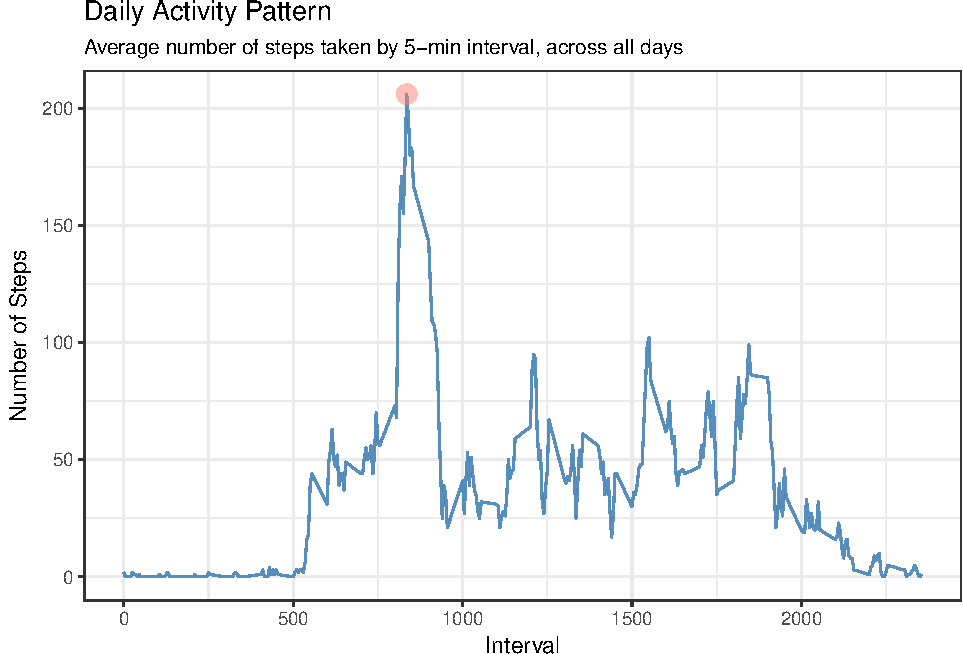
\includegraphics{figure/activity pattern-1} \end{center}

In the figure, we can observe a peak (maximum value) in the number of
steps taken, 206, in the interval 835.

\subsection{Imputing missing values}\label{imputing-missing-values}

\begin{verbatim}
Instructions:
Note that there are a number of days/intervals where there are missing values (coded as `NA`). The presence of missing days may introduce bias into some calculations or summaries of the data.
1. Calculate and report the total number of missing values in the dataset (i.e. the total number of rows with `NA`s).
2. Devise a strategy for filling in all of the missing values in the dataset. The strategy does not need to be sophisticated. For example, you could use the mean/median for that day, or the mean for that 5-minute interval, etc.
3. Create a new dataset that is equal to the original dataset but with the missing data filled in.
\end{verbatim}

\begin{Shaded}
\begin{Highlighting}[]
\NormalTok{nas.df <-}\StringTok{ }\NormalTok{activity.data }\OperatorTok\StringTok{ }\KeywordTok{sapply}\NormalTok{(is.na) }\OperatorTok\StringTok{ }\KeywordTok{tbl_df}\NormalTok{() }\OperatorTok\StringTok{ }\KeywordTok{summarise}\NormalTok{(}\DataTypeTok{Steps =} \KeywordTok{sum}\NormalTok{(steps), }
    \DataTypeTok{Date =} \KeywordTok{sum}\NormalTok{(date), }\DataTypeTok{Interval =} \KeywordTok{sum}\NormalTok{(interval))}

\KeywordTok{row.names}\NormalTok{(nas.df) <-}\StringTok{ }\KeywordTok{c}\NormalTok{(}\StringTok{"Number of NAs"}\NormalTok{)}

\NormalTok{nas.df }\OperatorTok\StringTok{ }\KeywordTok{kable}\NormalTok{(}\DataTypeTok{caption =} \StringTok{"Number of Missing Values of each Variable"}\NormalTok{, }\DataTypeTok{align =} \StringTok{"c"}\NormalTok{)}
\end{Highlighting}
\end{Shaded}

\begin{longtable}[]{@{}lccc@{}}
\caption{Number of Missing Values of each Variable}\tabularnewline
\toprule
& Steps & Date & Interval\tabularnewline
\midrule
\endfirsthead
\toprule
& Steps & Date & Interval\tabularnewline
\midrule
\endhead
Number of NAs & 2304 & 0 & 0\tabularnewline
\bottomrule
\end{longtable}

First, we want to know how many missing our data set has; in this case,
there are 2304 missing values, in total. The detail of the missing
values for each variable is shown in the table above

In the assignment instructions, we are required to devise a simple
strategy to impute missing values. The strategy that we'll follow is,
indeed, simple:

\begin{enumerate}
\def\labelenumi{\alph{enumi}.}
\tightlist
\item
  Get the trimmed mean of the number of steps (exclude the 10\% most
  extreme observations) by 5-min interval.
\item
  Joining the original data set with NAs and the data set of mean steps
  by 5-min interval.
\item
  Substitute NAs with the corresponding mean value.
\item
  Cleaning the data frame.
\end{enumerate}

\begin{Shaded}
\begin{Highlighting}[]
\NormalTok{non.NA <-}\StringTok{ }\NormalTok{activity.data }\OperatorTok\StringTok{ }\KeywordTok{group_by}\NormalTok{(interval) }\OperatorTok\StringTok{ }\KeywordTok{summarise}\NormalTok{(}\DataTypeTok{steps =} \KeywordTok{round}\NormalTok{(}\KeywordTok{mean}\NormalTok{(steps, }
    \DataTypeTok{na.rm =} \OtherTok{TRUE}\NormalTok{, }\DataTypeTok{trim =} \FloatTok{0.05}\NormalTok{)))}


\NormalTok{imp.activity.data <-}\StringTok{ }\KeywordTok{full_join}\NormalTok{(}\DataTypeTok{x =}\NormalTok{ activity.data, }\DataTypeTok{y =}\NormalTok{ non.NA, }\DataTypeTok{by =} \StringTok{"interval"}\NormalTok{) }\OperatorTok\StringTok{ }
\StringTok{    }\KeywordTok{mutate}\NormalTok{(}\DataTypeTok{steps =} \KeywordTok{ifelse}\NormalTok{(}\DataTypeTok{test =} \KeywordTok{is.na}\NormalTok{(steps.x), }\DataTypeTok{yes =}\NormalTok{ steps.y, }\DataTypeTok{no =}\NormalTok{ steps.x)) }\OperatorTok\StringTok{ }
\StringTok{    }\KeywordTok{select}\NormalTok{(steps, date, interval)}
\end{Highlighting}
\end{Shaded}

The histogram of the total number of steps taken per day doesn't change
much.

\begin{Shaded}
\begin{Highlighting}[]
\NormalTok{steps.day.df <-}\StringTok{ }\NormalTok{imp.activity.data }\OperatorTok\StringTok{ }\KeywordTok{group_by}\NormalTok{(date) }\OperatorTok\StringTok{ }\KeywordTok{summarise}\NormalTok{(}\DataTypeTok{steps =} \KeywordTok{sum}\NormalTok{(steps))}

\NormalTok{mean.median.steps <-}\StringTok{ }\NormalTok{steps.day.df }\OperatorTok\StringTok{ }\KeywordTok{summarise}\NormalTok{(}\DataTypeTok{Mean =} \KeywordTok{round}\NormalTok{(}\KeywordTok{mean}\NormalTok{(steps, }\DataTypeTok{na.rm =} \OtherTok{TRUE}\NormalTok{)), }
    \DataTypeTok{Median =} \KeywordTok{round}\NormalTok{(}\KeywordTok{median}\NormalTok{(steps, }\DataTypeTok{na.rm =} \OtherTok{TRUE}\NormalTok{))) }\OperatorTok\StringTok{ }\KeywordTok{gather}\NormalTok{()}

\KeywordTok{ggplot}\NormalTok{(}\DataTypeTok{data =}\NormalTok{ steps.day.df, }\DataTypeTok{mapping =} \KeywordTok{aes}\NormalTok{(}\DataTypeTok{x =}\NormalTok{ steps, }\DataTypeTok{y =}\NormalTok{ ..density..)) }\OperatorTok{+}\StringTok{ }\KeywordTok{geom_histogram}\NormalTok{(}\KeywordTok{aes}\NormalTok{(}\DataTypeTok{weight =}\NormalTok{ steps), }
    \DataTypeTok{fill =} \StringTok{"steelblue"}\NormalTok{, }\DataTypeTok{colour =} \StringTok{"white"}\NormalTok{, }\DataTypeTok{alpha =} \FloatTok{0.8}\NormalTok{) }\OperatorTok{+}\StringTok{ }\KeywordTok{geom_density}\NormalTok{(}\DataTypeTok{fill =} \StringTok{"steelblue"}\NormalTok{, }
    \DataTypeTok{colour =} \OtherTok{NA}\NormalTok{, }\DataTypeTok{alpha =} \FloatTok{0.2}\NormalTok{) }\OperatorTok{+}\StringTok{ }\KeywordTok{ggtitle}\NormalTok{(}\KeywordTok{list}\NormalTok{(}\DataTypeTok{title =} \StringTok{"Total Number of Steps"}\NormalTok{, }\DataTypeTok{subtitle =} \StringTok{"Distribution of Total Number of Steps Taken Each Day"}\NormalTok{, }
    \DataTypeTok{x =} \StringTok{"Steps"}\NormalTok{, }\DataTypeTok{y =} \StringTok{"Density"}\NormalTok{)) }\OperatorTok{+}\StringTok{ }\KeywordTok{geom_vline}\NormalTok{(}\DataTypeTok{data =}\NormalTok{ mean.median.steps, }\KeywordTok{aes}\NormalTok{(}\DataTypeTok{xintercept =}\NormalTok{ value, }
    \DataTypeTok{linetype =}\NormalTok{ key), }\DataTypeTok{size =} \FloatTok{0.5}\NormalTok{, }\DataTypeTok{alpha =} \FloatTok{0.8}\NormalTok{, }\DataTypeTok{colour =} \KeywordTok{c}\NormalTok{(}\StringTok{"salmon"}\NormalTok{, }\StringTok{"royalblue"}\NormalTok{)) }\OperatorTok{+}\StringTok{ }
\StringTok{    }\KeywordTok{scale_linetype_discrete}\NormalTok{(}\DataTypeTok{name =} \StringTok{"Number of Steps"}\NormalTok{) }\OperatorTok{+}\StringTok{ }\KeywordTok{theme_bw}\NormalTok{()}
\end{Highlighting}
\end{Shaded}

\begin{center}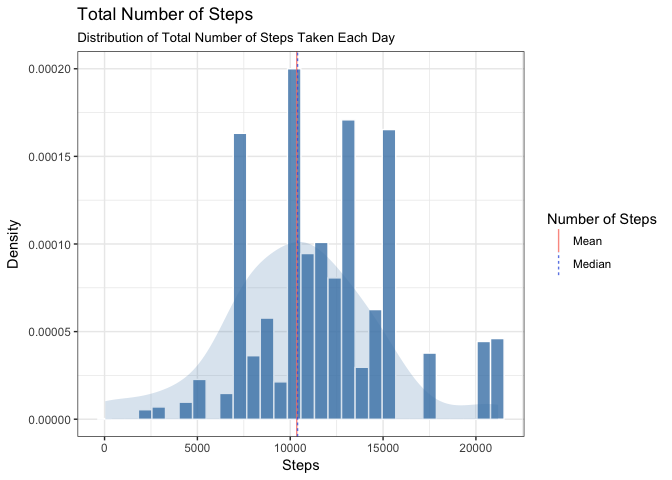
\includegraphics{figure/histogram of complete steps-1} \end{center}

With the chosen imputation strategy, there were no changes in the median
and mean number of the steps taken per day.

\begin{Shaded}
\begin{Highlighting}[]
\NormalTok{steps.day.df }\OperatorTok\StringTok{ }\KeywordTok{summarise}\NormalTok{(}\StringTok{`}\DataTypeTok{Mean number of steps taken per day}\StringTok{`}\NormalTok{ =}\StringTok{ }\KeywordTok{round}\NormalTok{(}\KeywordTok{mean}\NormalTok{(steps, }
    \DataTypeTok{na.rm =} \OtherTok{TRUE}\NormalTok{)), }\StringTok{`}\DataTypeTok{Median number of steps taken per day}\StringTok{`}\NormalTok{ =}\StringTok{ }\KeywordTok{round}\NormalTok{(}\KeywordTok{median}\NormalTok{(steps, }
    \DataTypeTok{na.rm =} \OtherTok{TRUE}\NormalTok{))) }\OperatorTok\StringTok{ }\KeywordTok{kable}\NormalTok{(}\DataTypeTok{align =} \StringTok{"c"}\NormalTok{)}
\end{Highlighting}
\end{Shaded}

\begin{longtable}[]{@{}cc@{}}
\toprule
Mean number of steps taken per day & Median number of steps taken per
day\tabularnewline
\midrule
\endhead
10350 & 10395\tabularnewline
\bottomrule
\end{longtable}

\subsection{Are there differences in activity patterns between weekdays
and
weekends?}\label{are-there-differences-in-activity-patterns-between-weekdays-and-weekends}

\begin{verbatim}
Instructions:
For this part the `weekdays()` function may be of some help here. Use the dataset with the filled-in missing values for this part.
1. Create a new factor variable in the dataset with two levels -- "weekday" and "weekend" indicating whether a given date is a weekday or weekend day.
2. Make a panel plot containing a time series plot (i.e. type = "l") of the 5-minute interval (x-axis) and the average number of steps taken, averaged across all weekday days or weekend days (y-axis).
\end{verbatim}

\begin{Shaded}
\begin{Highlighting}[]
\NormalTok{avg.steps.weekday <-}\StringTok{ }\NormalTok{imp.activity.data }\OperatorTok\StringTok{ }\KeywordTok{mutate}\NormalTok{(}\DataTypeTok{weekday.end =} \KeywordTok{ifelse}\NormalTok{(}\DataTypeTok{test =} \KeywordTok{weekdays}\NormalTok{(date, }
    \DataTypeTok{abbreviate =} \OtherTok{TRUE}\NormalTok{) }\OperatorTok\StringTok{ }\KeywordTok{c}\NormalTok{(}\StringTok{"Sat"}\NormalTok{, }\StringTok{"Sun"}\NormalTok{), }\DataTypeTok{yes =} \StringTok{"Weekend"}\NormalTok{, }\DataTypeTok{no =} \StringTok{"Weekday"}\NormalTok{)) }\OperatorTok\StringTok{ }
\StringTok{    }\KeywordTok{group_by}\NormalTok{(interval, weekday.end) }\OperatorTok\StringTok{ }\KeywordTok{summarise}\NormalTok{(}\DataTypeTok{steps =} \KeywordTok{round}\NormalTok{(}\KeywordTok{mean}\NormalTok{(steps, }\DataTypeTok{na.rm =} \OtherTok{TRUE}\NormalTok{)))}

\NormalTok{maxima.steps <-}\StringTok{ }\NormalTok{avg.steps.weekday }\OperatorTok\StringTok{ }\KeywordTok{group_by}\NormalTok{(weekday.end) }\OperatorTok\StringTok{ }\KeywordTok{top_n}\NormalTok{(}\DecValTok{1}\NormalTok{, steps)}

\KeywordTok{ggplot}\NormalTok{(}\DataTypeTok{data =}\NormalTok{ avg.steps.weekday, }\DataTypeTok{mapping =} \KeywordTok{aes}\NormalTok{(}\DataTypeTok{x =}\NormalTok{ interval, }\DataTypeTok{y =}\NormalTok{ steps)) }\OperatorTok{+}\StringTok{ }\KeywordTok{geom_line}\NormalTok{(}\DataTypeTok{colour =} \StringTok{"steelblue"}\NormalTok{, }
    \DataTypeTok{alpha =} \FloatTok{0.9}\NormalTok{) }\OperatorTok{+}\StringTok{ }\KeywordTok{facet_grid}\NormalTok{(weekday.end }\OperatorTok{~}\StringTok{ }\NormalTok{.) }\OperatorTok{+}\StringTok{ }\KeywordTok{geom_point}\NormalTok{(}\DataTypeTok{data =}\NormalTok{ maxima.steps, }
    \DataTypeTok{mapping =} \KeywordTok{aes}\NormalTok{(}\DataTypeTok{x =}\NormalTok{ interval, }\DataTypeTok{y =}\NormalTok{ steps, }\DataTypeTok{group =}\NormalTok{ weekday.end), }\DataTypeTok{alpha =} \FloatTok{0.5}\NormalTok{, }\DataTypeTok{size =} \DecValTok{4}\NormalTok{, }
    \DataTypeTok{colour =} \StringTok{"salmon"}\NormalTok{) }\OperatorTok{+}\StringTok{ }\KeywordTok{ggtitle}\NormalTok{(}\KeywordTok{list}\NormalTok{(}\DataTypeTok{title =} \StringTok{"Activity Patterns in Weekdays and Weekends"}\NormalTok{, }
    \DataTypeTok{y =} \StringTok{"Number of Steps"}\NormalTok{, }\DataTypeTok{x =} \StringTok{"Interval"}\NormalTok{)) }\OperatorTok{+}\StringTok{ }
\KeywordTok{theme_bw}\NormalTok{()}
\end{Highlighting}
\end{Shaded}

\begin{center}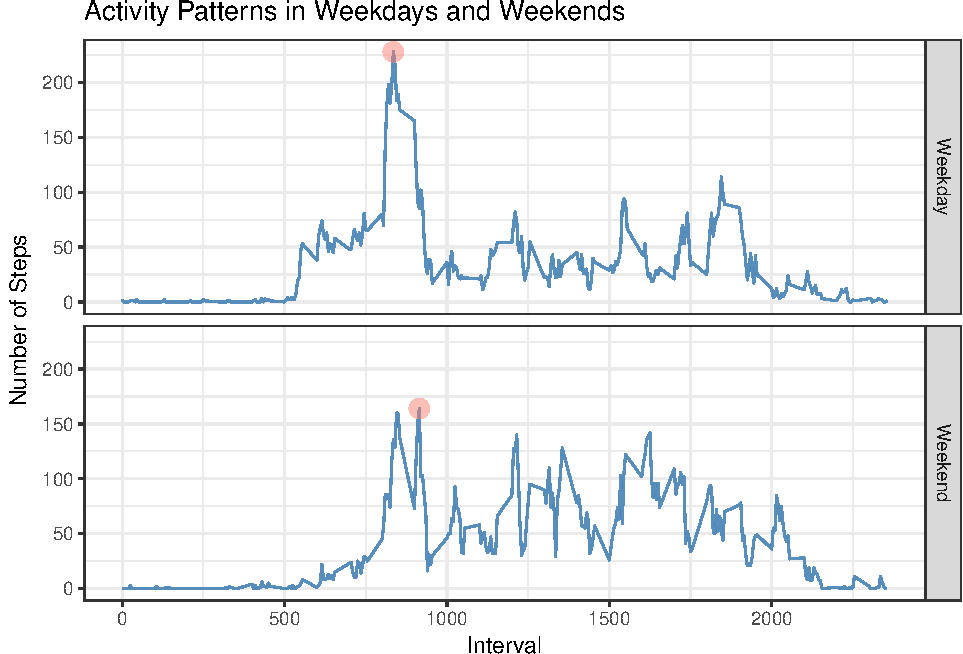
\includegraphics{figure/diff activity patterns weekday-end-1} \end{center}

The maxima number of steps during weekend and weekdays are notoriously
different, as can be seen in the figure above. The peak of activity
during the weekdays is 228 steps, which happens in the 835 interval;
while the peak of activity during the weekends is 164 steps, which
happens in the 915 interval.


\end{document}
